%Stuff to insert:
%\begin{itemize}
%	\item Generation of random points (details)
%	\item Noise generation on GPU (caveats)
%	\item Sampling patterns (details)
%	\item Layered rendering (details)
%	\item Shadow mapping (for lights) (details)
%	\item Ping-ponging and accumulation (details)
%	\item Texture Views and mipmap generation (memory optimization) (caveats)
%	\item Engine structure (no)
%	\item Extension: compute shaders
%	\item Extension: image load store (meh)
%	\item Extension: subroutines (meh)
%	\item Sampling colormap
%	\item Alternative: voxelization
%	\item Multiple lights
%	\item Different types of light
%	\item Skyboxes
%\end{itemize}


%Caveats:
%\begin{itemize}
%	\item Oversampling issues in final combinaiton (multisampling of depth map)
%	\item Combination delta
%	\item Shadow bias
%  \item Random rotation
	
%\end{itemize}

\chapter{Implementation}

In this chapter, we will introduce the implementation details of our method. The difference between this chapter and the previous one is that the concepts introduced in the method chapter are easily adaptable to any kind of implementation environment, while in this chapter we focus on a GPU-oriented implementation. First, we will give a general outline of our algorithm. Then, we will take each one of the single parts of the algorithm and discuss them separately. After introducing the details of the algorithm, we will discuss some caveats that are necessary in order to eliminate defects and artifacts in our algorithm. Finally, we will discuss our implementation, introducing some possible implementation alternatives in order to compare them in the result section.

\section{Environment}

In order to better contextualize some of the choices and the code parts that will be introduced in this section, we will first introduced the environment used in our implementation. The method we are going to discuss was made using the OpenGL API, version 4.3 (released in August 2012), a multi-platform API used for rendering 2D and 3D accelerated graphics. With the OpenGL API comes together GLSL, the OpenGL Shading Language, used for writing pieces of code to be run on the GPU, called \emph{shaders}. Our method uses some advanced features of OpenGL 4.3, so it is not immediately portable to previous generation hardware, and runs only on high-end modern GPUs. On the CPU side, we use an extended framework based on Qt, a C++ library that allows to create OpenGL contexts and graphical interfaces in an easy way.

In this chapter, we describe the implementation details of our technique, using the approximation of the rendering equation introduced in the previous chapter. We start by giving a rather generic introduction of our algorithm, introducing then all the implementation details. 


%\section{Requirements}
%
%Our algorithm, in order to be generic and applicable to a wide range of situations must meet some requirements. 
%
%
%\begin{itemize}
  %\item The algorithm should be \emph{accurate}, so that the renderings are as close as possible to reference images generated using a offline Monte-Carlo simulation. 
	%\item The algorithm should be \emph{fast}, executing at interactive frame rates.
	%\item The algorithm should be \emph{uv-independent}, not relying on a pre-made UV mapping of the object in order to being able to perform. The algorithm should work only if basic geometric features are provided (vertices and normals).
	%\item The algorithm should be \emph{adaptable}, handling in real-time dynamic light changes and object deformations. So it will not possible to use light baking or geometry form factors.
%\end{itemize}
%
%If it is not possible to satisfy all the previous within the strict constraints of real-time rendering, we want to create an algorithm that gets as close as possible to the requested result. The algorithm should progressively progressively improve and converge to an accurate result whenever possible (e.g. when the light in the scene is not changing).

\section{Algorithm overview}

By keeping the limitations presented in the previous chapter in mind TODO, we introduce our four pass algorithm. The algorithm is inspired by \emph{translucent shadow maps} TODO, that we presented in chapter TODO. The general idea is to first render the scene from the light point of view, then place the disk we discussed in the method chapter TODO directly on the generated texture. We use many directions in order to capture all the sides of the object. In this section, we will assume to only have one directional light $L_d$, $\vomega_d$ and one not-deformable object in the scene. We will discuss later how to extend the method to multiple light sources.

\textbf{Step 1 - Light buffer} \\

In the first step, positions and normals of the object are rendered into a texture from the light point of view. As in standard shadow mapping we create and store a matrix to convert between world space and texture light space. Depth testing in this step is enabled.

\begin{figure}[!ht]
\centering
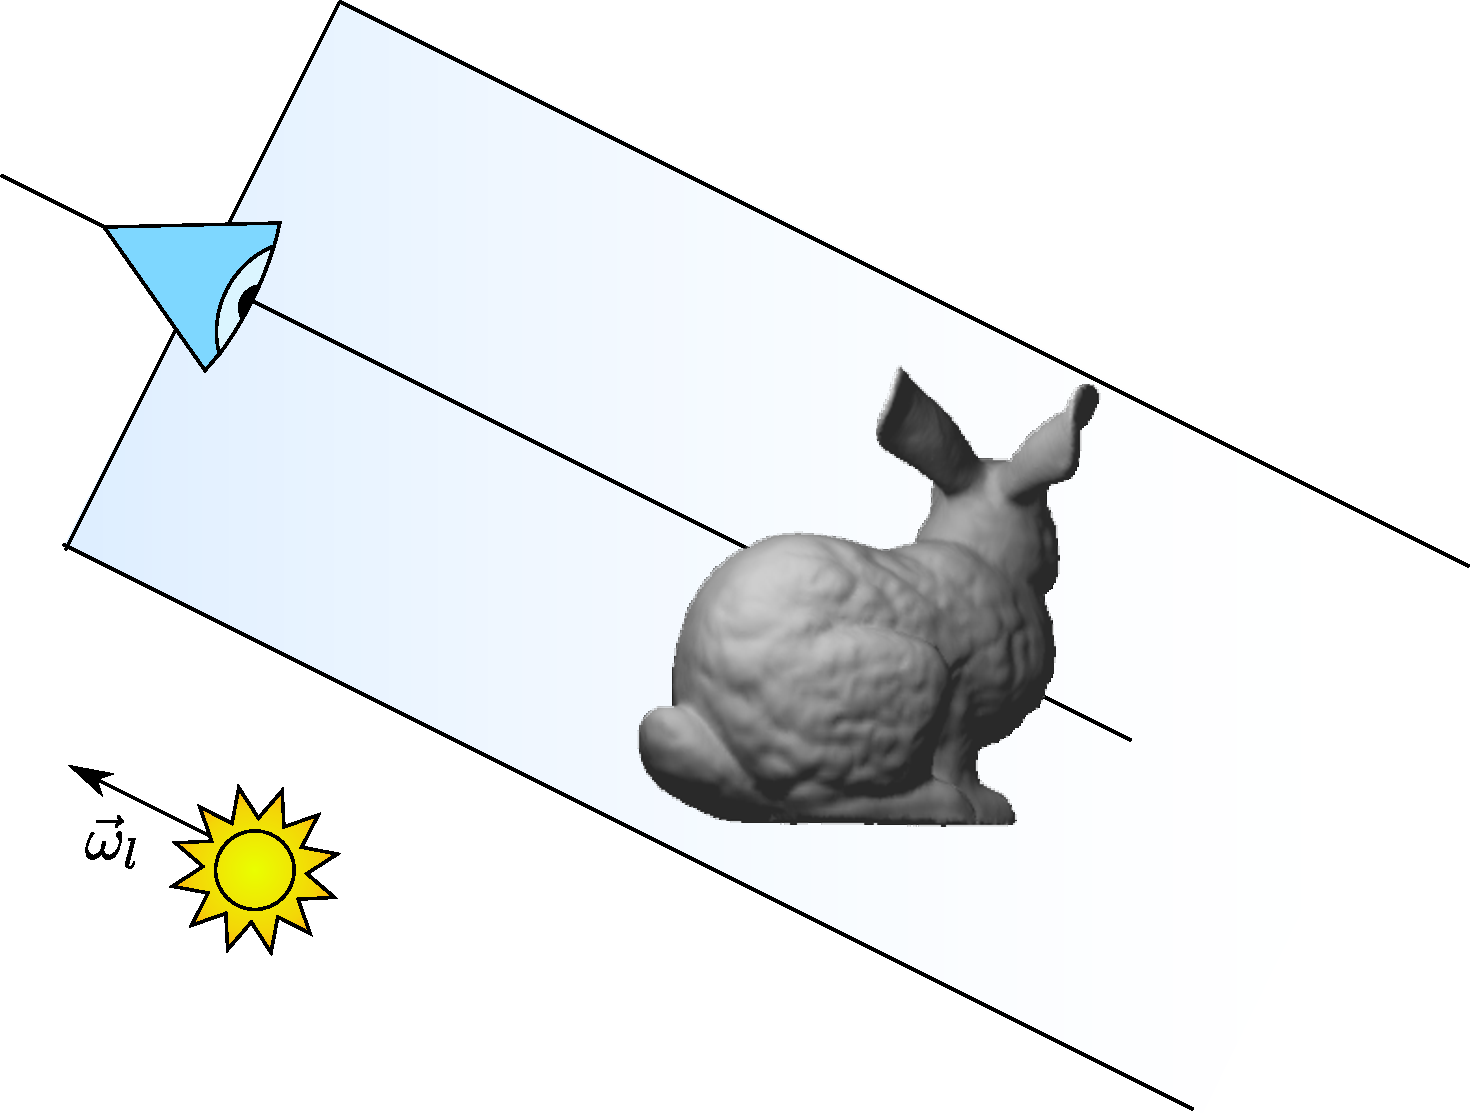
\includegraphics[width=0.8 \linewidth]{images/method/step1.pdf}
\caption{Render to G-buffer. Note that the frustum and the light direction are aligned.}
\label{fig:step1}
\end{figure} 


\begin{figure}
\centering
\subfloat[{Vertex buffer}]{
  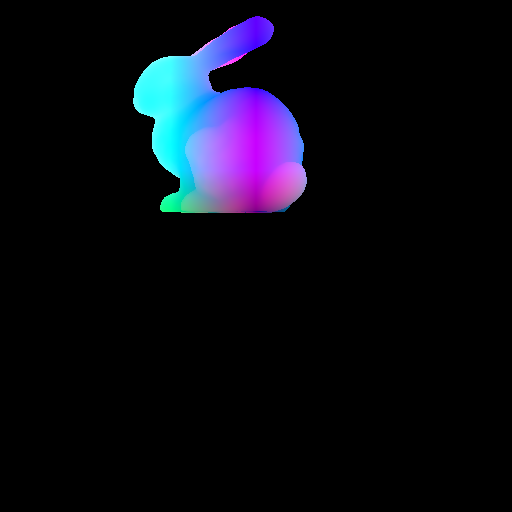
\includegraphics[width=0.5 \linewidth]{images/method/vertices.png}
  \label{fig:vbuff}
}
\subfloat[{Normal buffer}]{
  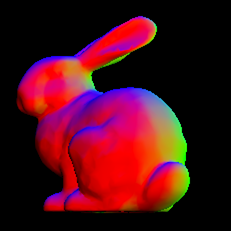
\includegraphics[width=0.5 \linewidth]{images/method/normals.png}
  \label{fig:nbuff}
} 
\label{fig:lightbuffers}
\caption{State of the vertex and normal buffer after rendering from a directional light. The model used was the Stanford bunny from the Standford 3D Scanning repository.}
\end{figure}

\FloatBarrier

\textbf{Step 2 - Render to radiance map} \\
In the second step, we render the object from $K$ different directions into a radiance map. The radiance map is organized as a layered texture, where each layer represents a direction. The points on which to place the cameras are chosen randomly. On each layer, we accumulate the result over different frames. On the rendering step, for each pixel that corresponds to an exitance point $\x_o$ the shader samples $N$ points from the texture rendered in the previous step. If the sampled point is valid, it is then used to calculate the BSSRDF and accumulate it in the resulting radiance map. So, this step calculates the following:

$$
R^{t,k}(\x_o) = L_d \sum_{i = 1}^N S(\x^{t,k}_i, \vomega^t_l, \x_o, \vomega_o) \exp\left(\sigma_{tr} r^{t,k}_i\right), \ \ t \in [0,T], \ \ k \in [0,K-1] 
\label{eq:evolution_step}
$$

\begin{figure}[!ht]
\centering
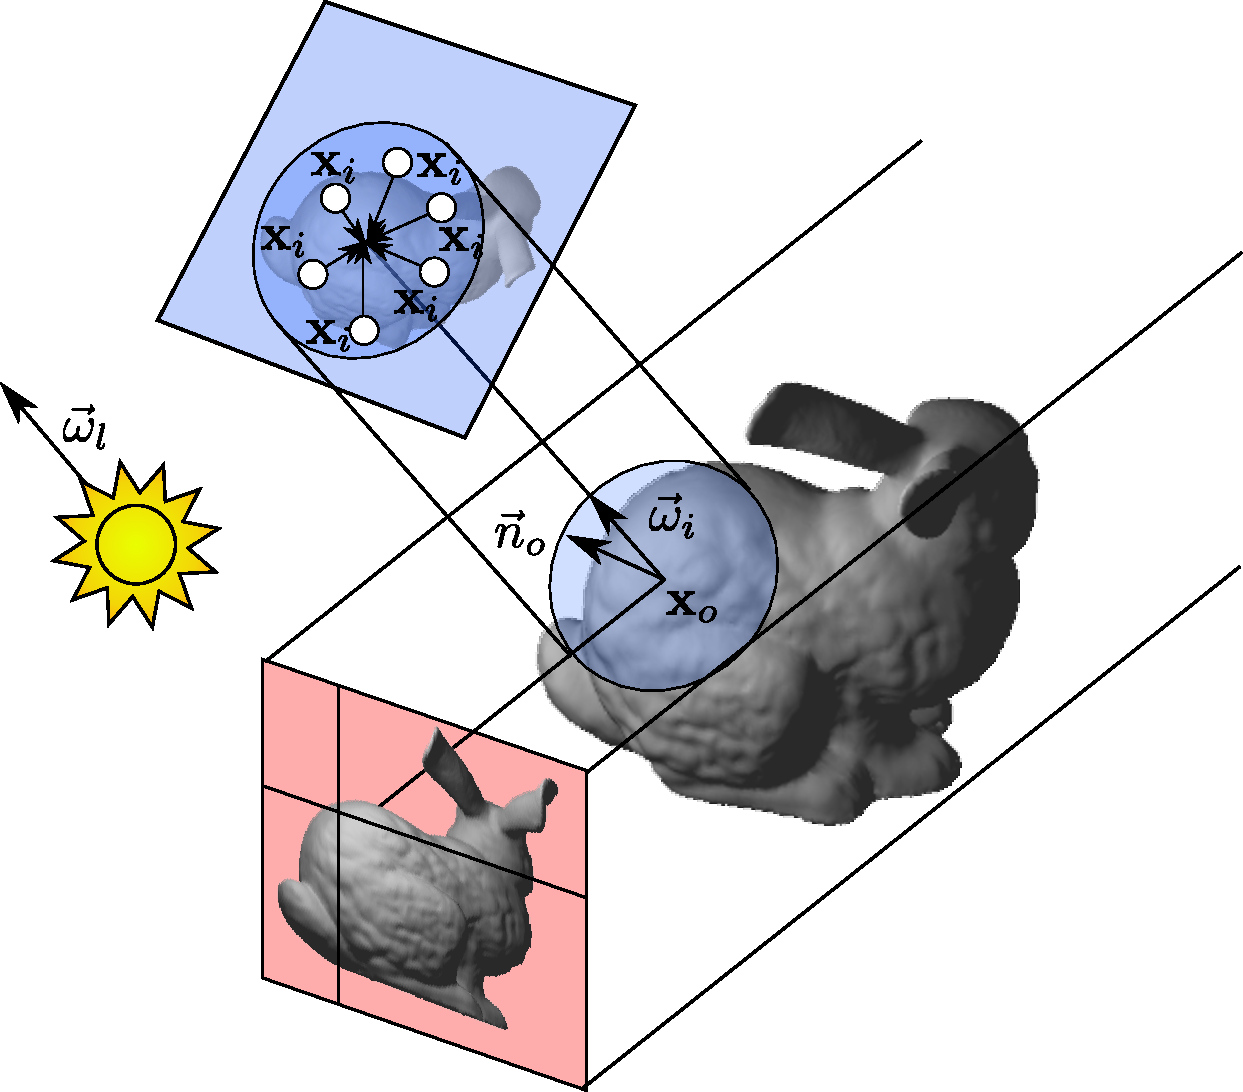
\includegraphics[width=0.9 \linewidth]{images/method/step2_improved.pdf}
\caption{Render to the radiance map. When we render the point $\x_o$, the position in the lightmap is calculated and the values $\x_i$ in the samples are calculated and summed over.}
\label{fig:step2}
\end{figure} 

Where we recall that we have introduced an exponential term in order to compensate for the exponential displacement of the sampling pattern. We introduced also a time $t$ parameter, that represents the fact that the result change over time, and a $k$ parameter, that represents the current direction we are rendering to. We can see how we are rendering a point from one of the considered directions in Figure \ref{fig:stepfrustum}. Also in this case, the texture space - world space conversion matrices are stored and prepared to be reused in the final combination step. 

We can appreciate that rendering the light from the camera point of view comes with two important advantages:

\begin{itemize}
	\item If the disk is placed in texture space, it is automatically oriented towards the light direction, that is $\vomega_d = \vomega_l$.
	\item The light renders in the texture only the points directly visible from it, that are also the points where the light radiance is maximum. In addition, if we sample the lightmap on any point, we get the corresponding vertex that is closest to the light.
\end{itemize}

This two factors allows us to sample the most optimal point and direction in where to place the disk, as we described it in section TODO.
 
\begin{figure}[!ht]
\centering
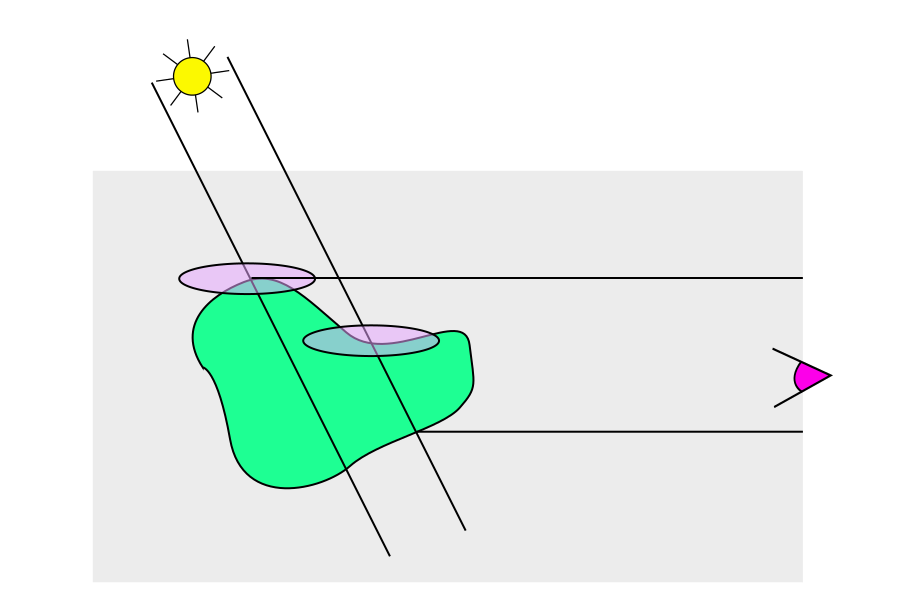
\includegraphics[width=\linewidth]{images/method/step2}
\caption{Render to cubemap, side view. The gray area represents the frustum of the current direction's camera (orthographic). We have three different cases of a point on the surface: $\x_o^1$ is visible from both the light and the camera, so the disk is placed on it. $\x_o^2$ is visible from the camera but not from the light, so the disk is placed in the closest position to the light. $\x_o^3$ is not visible from the camera, so it is discarded.}
\label{fig:stepfrustum}
\end{figure} 

In this step, there is an accumulation process going on:

$$
\tilde{R}^{t,k} = \sum_{i = 0}^{t-1} R^{i,k} + R^{t,k} = \tilde{R}^{t-1, k} + R^{t,k}
$$

$\tilde{R}$ here represents the actual value that is stored in the texture or loaded from the previous one. We need an accumulation process in order to deal with the fact that the result from the previous computation are not reaching a satisfying result within one frame, so they need to be accumulated over a period of $T$ frames in order to reach converge to an appreciable result. In order to do this, the sampled points need to change on different frames (see section TODO) for more details. 

Naturally, the accumulation process works only if the scene does not change. A change can be a relative change of positions between the points on the model and the light, so if the model gets rotated or scaled (translation for directional lights is irrelevant), the accumulated result has to be discarded and the accumulation started all over. The cameras are locked with the model, so the pixels are always aligned irregardless of the model matrix of the object. This is why in equation \ref{eq:evolution_step} the dependence from time of the point $\x_o$ and $\vomega_o$ have been dropped. Obviously, the dependence must be reintroduced in case we are dealing with deformable objects.
 
\textbf{Step 3 - Combination} \\
In this step, we have the final render of our model. While all the previous steps were not rendering anything in the scene (making a render-to-texture), in this scene we do an actual rendering of the model. Using the matrices prepared in the previous step, for each fragment on the surface we sample all the layers in the texture as illustrated in Figure \ref{fig:step3}. In order to do this, we need also to sample the depth map generated in the previous step. We can define this sampling as a visibility function to test if a point $\x$ belongs to layer $k$:

$$
V^k(\x) = \begin{cases}
1 & \text{if $\x$ is visible from the $k$th camera} \\
0 & \text{otherwise}
\end{cases}
$$
Given this function, we can simply represent the outgoing radiance by simply averaging the summation over the $K$ layers:

$$
L_{SS}^t(\mathbf{x}) = \frac{A_c}{N (t + 1)} \frac{\displaystyle\sum_{k = 0}^{K-1}V^k(\x) \tilde{R}^{t,k}(\mathbf{x})}{\displaystyle\sum_{k = 0}^{K-1}V^k(\x)}
$$

The first factor $\frac{1}{t + 1}$ is to average over the number of frames, while the second is the average area of a sample in the circle $\frac{A_c}{N}$, that is necessary to complete the equation as described in TODO. We note that we tried to move all the layer-independent computation into the final computation step, in order to save as much performance as possible. 

\begin{figure}[!ht]
\centering
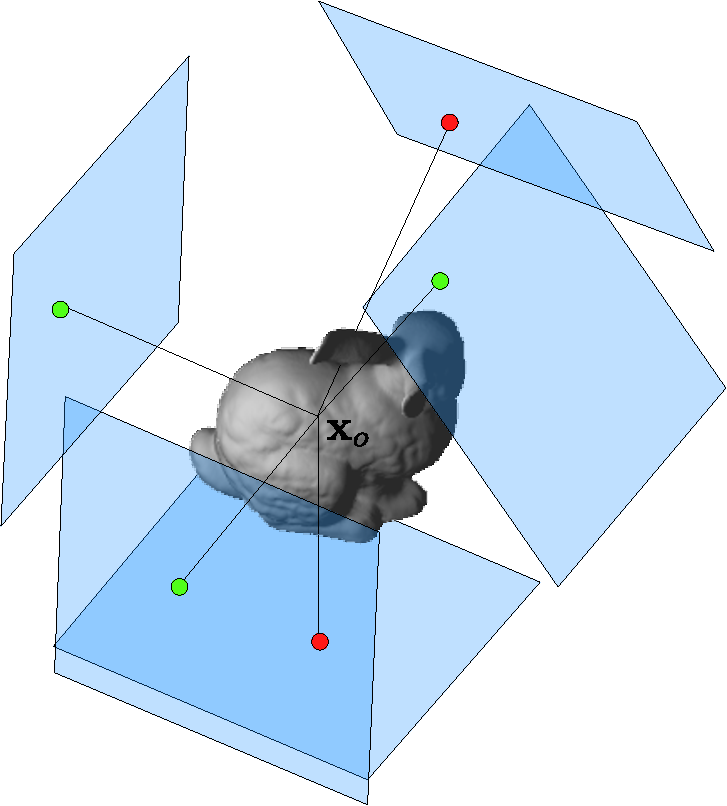
\includegraphics[width=0.6 \linewidth]{images/method/combination.pdf}
\caption{Final combination step. The blue quads indicates each one of the radiance map layers, as seen from their direction. We can see that in the point $\x_o$ the contribution from three faces (green dots) is considered. For the remaining two faces (red dots), the contribution is not considered as the point is not visible.}
\label{fig:step3}
\end{figure} 

We are not done yet, as for now we have computed the radiance only deriving from subsurface scattering. For finally describing the illumination of our scene, we need also to include a factor based on the surface reflection. Since the subsurface scattering radiance is already multiplied by a transmittance Fresnel term (in the BSSRDF equation in TODO) $T(\eta,\vomega_o)$ we the reflection color multiplied by the converse transmission term $1 - T(\eta,\vomega_o)$:

$$
L^t(\x, \vomega_o) = L_{SS}^t(\x) + (1 - T(\eta,\vomega_o)) L_i(\x, \vomega_o - 2 (\vomega_o \cdot \vec{n}) \vec{n})
$$

$L_i$ can be the radiance coming from other objects or by an environment map. After this, we just need to perform gamma correction in order to get the final result. Given the gamma coefficient $\gamma$, we perform gamma correction by:

$$
L_{gamma}^t(\x, \vomega_o, \gamma) = L^t(\x,\vomega_o)^{\frac{1}{\gamma}}
$$

And we can finally send the radiance to the output device.

\section{Implementation details}
In this section, we will further expand the overview  given in the previous section adding further details. We organized this section in topics, rather than following the order given by the algorithm, since most of the topic we will introduce will be used in multiple places. We will point out where each topic will be used in the algorithm.

\subsection{Render-to-texture}
In a graphics API, and more specifically in OpenGL, all the output from a final shader stage is usually sent to the display device in order to be displayed on the screen. However, it is possible to redirect the output into another memory area of the GPU and reuse it for further computations. This allows to create complicated rendering techniques such as the ones described in this report. 

In OpenGL, is possible to redirect the output more specifically to a texture object. We can do this through a so-called \emph{framebuffer object} (FBO). A FBO is a complex collection of objects that allow offscreen rendering. A FBO has \emph{attachment points}, to which we can attach textures between the various things. A texture can be attached to one of the output color channels of the fragment shader (\gl{GL_COLOR_ATTACHMENT0}, \gl{GL_COLOR_ATTACHMENT1}, ...), to the depth buffer output (\gl{GL_DEPTH_ATTACHMENT}) or to the stencil buffer output (\gl{GL_STENCIL_ATTACHMENT}).

The connection between the framebuffer and the texture can be set in a initialization step. Afterwards, by simply binding the FBO we will render to the configured texture:

\begin{lstlisting}[language=C++,label=lst:rendertotextureinit,caption={Render to texture example, initilalization phase. Note the call to \gl{glFramebufferTexture2D}}]
GLuint tex,fbo;
// Generating texture
glGenTextures(1, &tex);
glBindTexture(GL_TEXTURE_2D, tex);
[...] // setting up texture parameters...
glTexImage2D(GL_TEXTURE_2D, 0, GL_RGBA16F, size, size, 0, GL_RGBA, GL_FLOAT, 0);


glGenFramebuffers(1,&fbo);

// connecting current fbo and texture
glBindFramebuffer(GL_DRAW_FRAMEBUFFER, fbo);
glFramebufferTexture2D(GL_DRAW_FRAMEBUFFER, GL_COLOR_ATTACHMENT0, GL_TEXTURE_2D, tex, 0);
glBindFramebuffer(GL_DRAW_FRAMEBUFFER, 0); //Binding back main framebuffer
\end{lstlisting}

\begin{lstlisting}[language=C++,label=lst:rendertotexturerender,caption={Render to texture example, rendering phase. Since we have not configured and FBO for depth and stencil buffers, depth testing and stencil should be disabled at this point.}]
glBindFramebuffer(GL_DRAW_FRAMEBUFFER, fbo);
GLenum buffers[] = {GL_COLOR_ATTACHMENT0};
glDrawBuffers(1, buffers);
[...] // draw model
\end{lstlisting}

\subsection{Layered rendering}
Layered rendering is a special feature used to render to a special type of texture called \emph{layered texture}. Let us take as an example the step 2 of our algorithm, where we need to render the object from $K$ different directions. A first approach to this would be to create $K$ 2D textures of type \gl{GL_TEXTURE_2D}, and perform $K$ draw calls, rebinding the texture on the current FBO each time. OpenGL, however, provides a way to do this faster, and with a single draw call, potentially reducing the rendering costs due to context switching.

\begin{figure}[!ht]
\centering
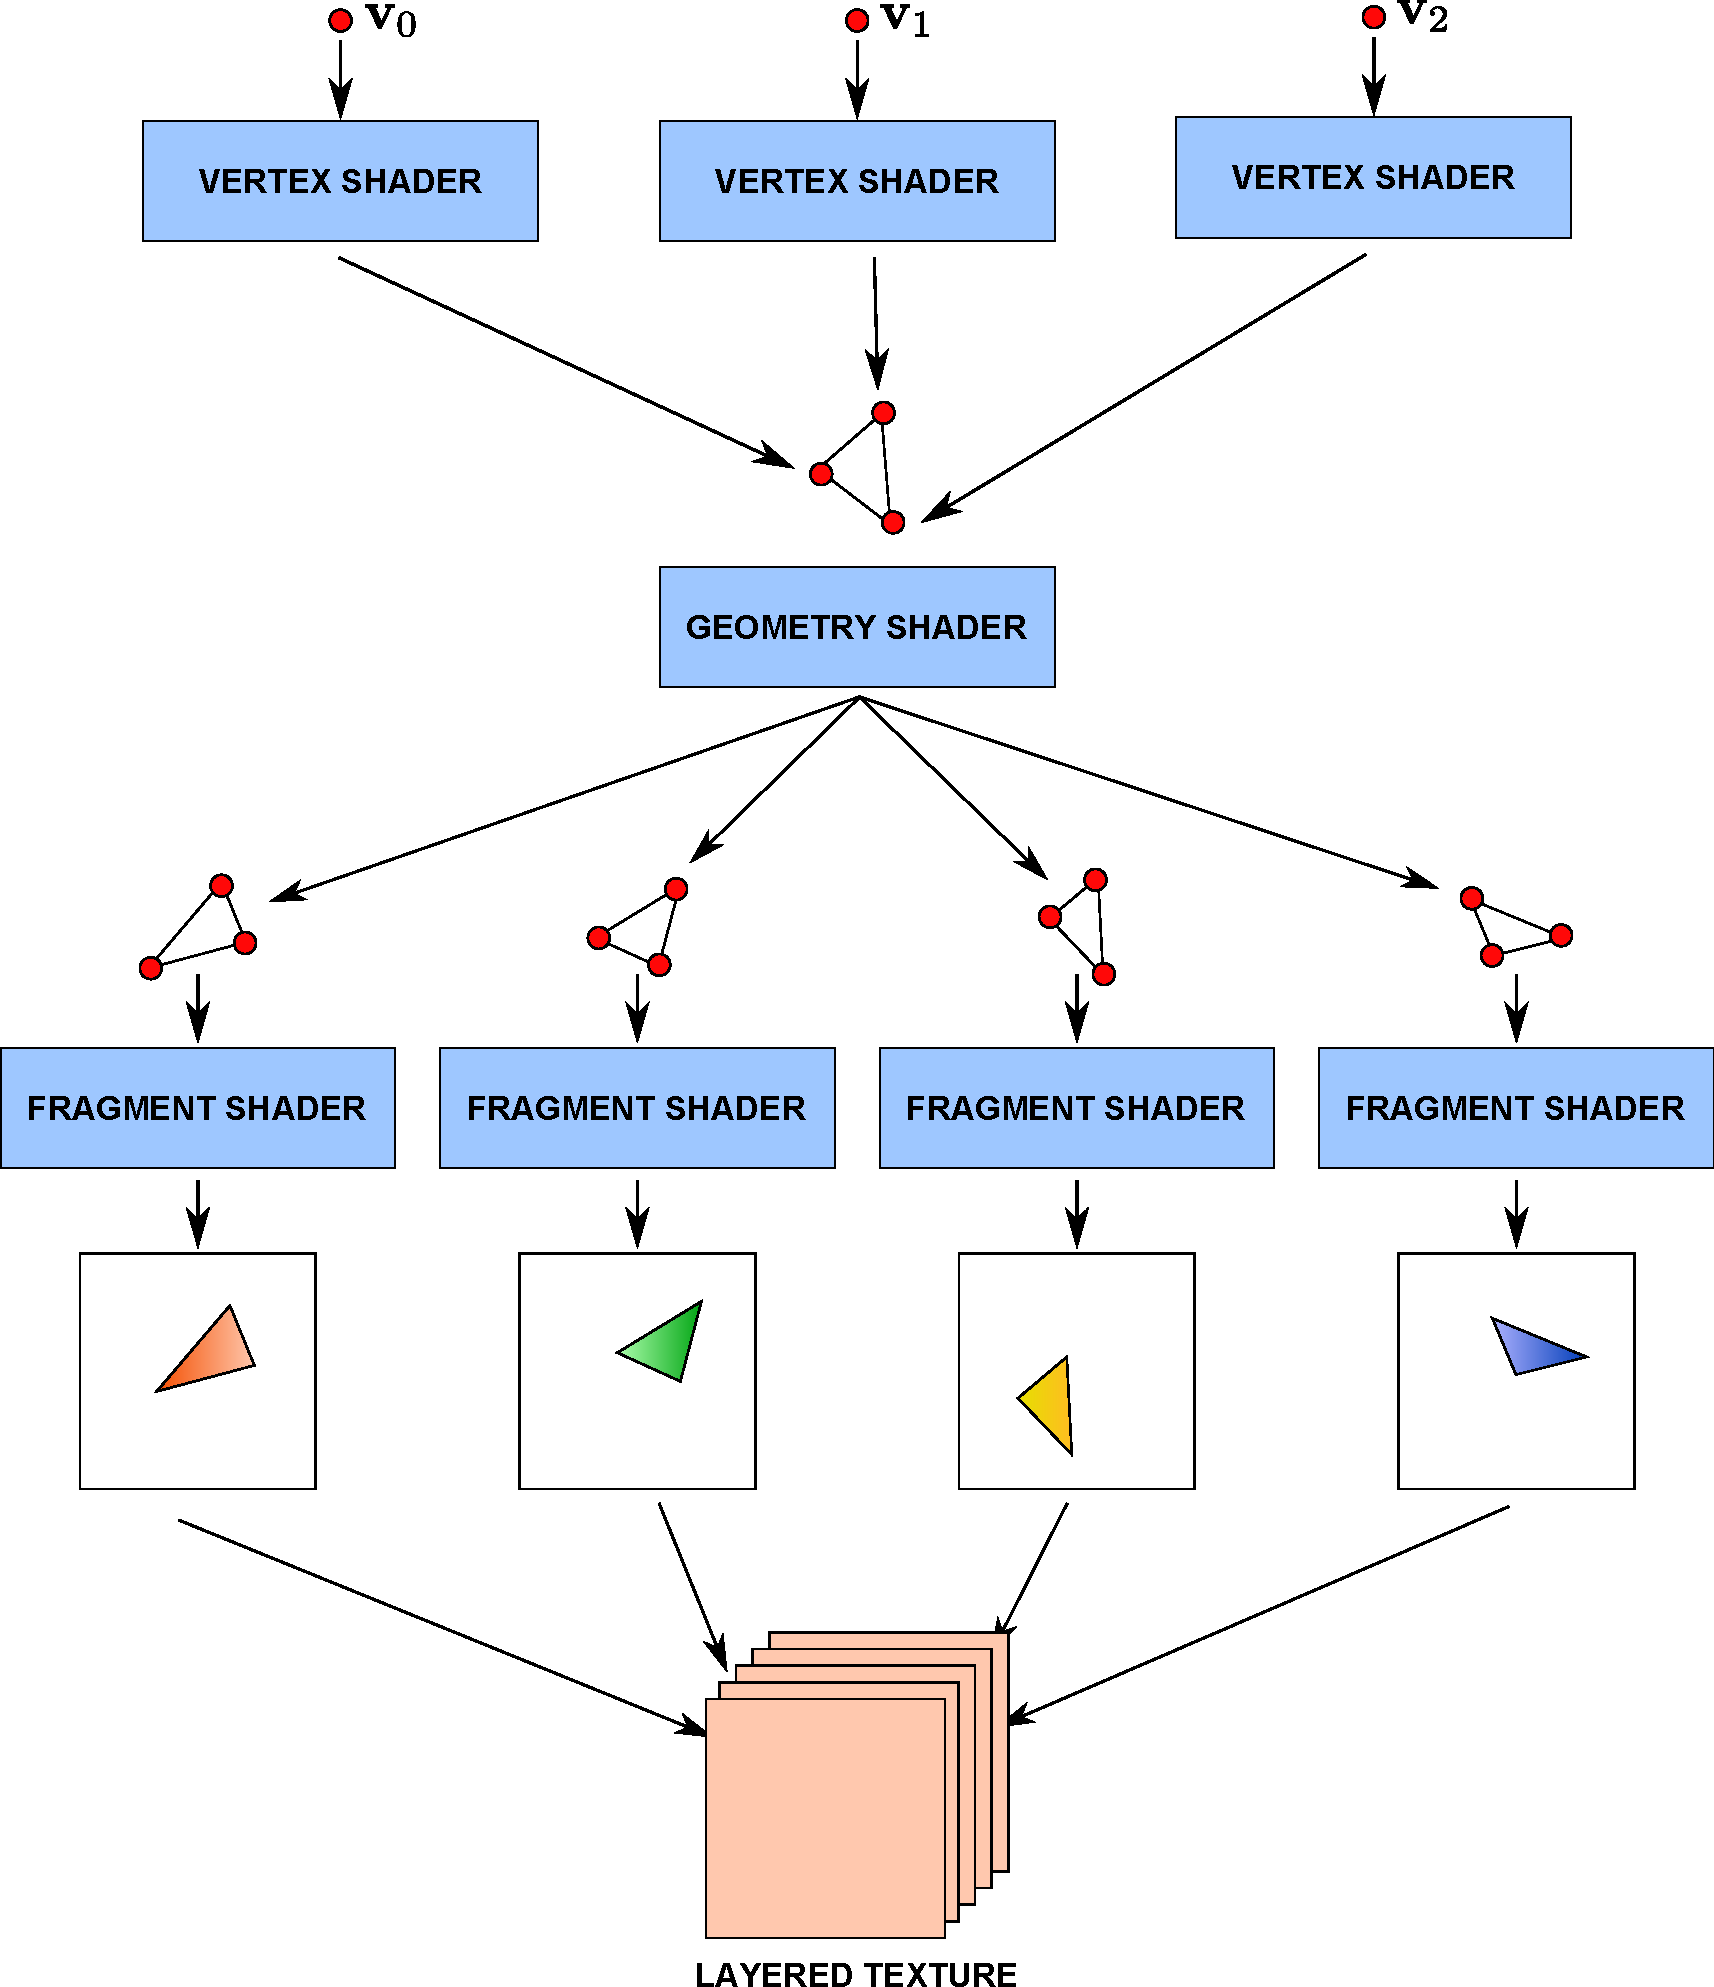
\includegraphics[width=\linewidth]{images/method/layered.pdf}
\caption{Diagram that illustrates layered rendering.}
\label{fig:step3}
\end{figure} 

We will use the OpenGL provided type \gl{GL_TEXTURE_2D_ARRAY}, that we initialize in the usual way, noting that an array texture should be initialized as a 3D texture. When binding it to an FBO, we use the generic \gl{glBindFramebufferTexture}:

\begin{lstlisting}[language=C++,label=lst:initarraytexture,caption={Initializing array texture. Note that the number of layers is passed to the \gl{glTexStorage3D} command.}]
GLuint fbo, arraytex;
glGenFramebuffers(1,&fbo);
glGenTextures(1, &arraytex);

glBindTexture(GL_TEXTURE_2D_ARRAY, arraytex);
[...] // setting up texture parameters, omitted
glTexStorage3D(GL_TEXTURE_2D_ARRAY, levels, GL_RGBA32F, size, size,layers);

glBindFramebuffer(GL_DRAW_FRAMEBUFFER, fbo);
glFramebufferTexture(GL_DRAW_FRAMEBUFFER, GL_COLOR_ATTACHMENT0, arraytex, 0);
\end{lstlisting}

In order to render to a layered texture, we need then to introduce a geometry shader. In our example, the difference between each layer is basically a different view matrix. So, we move the computation of the position, usually left to the vertex shader, to the geometry shader. We first introduce the code:

\begin{lstlisting}[language=GLSL,label=lst:arraygeomshader,caption={Geometry shader for layered rendering. The multiplication by the model matrix of vertex v is performed in the vertex shader (not shown).}]
#version 430
#define DIRECTIONS 16
layout(triangles) in;
layout(triangle_strip, max_vertices = 60) out;

uniform mat4 P;
uniform mat4 viewMatrices[DIRECTIONS];

void main(void)
{
    for(int i = 0; i < DIRECTIONS; i++)
    {
        gl_Layer = i;

        for(int k = 0; k < 3; k++)
        {
            vec4 v = gl_in[k].gl_Position;
            gl_Position = P * viewMatrices[i] * v;
            EmitVertex();
        }
        EndPrimitive();
    }
}
\end{lstlisting}

As we can see, we duplicate each one of the incoming triangles and then output it multiplied by a different view matrix. the \gl{EndPrimitive()} function ensures that the output triangles in the final triangle strip are separated. In order to render to a different layer each triangle, we need to set the special \gl{gl_Layer} variable to the layer we want to render before emitting the triangle. The whole process is illustrated in figure TODO.

\subsection{Accumulation buffers}

Often, during the rendering process, we would like to accumulate the result of a computation, in order to progressively update the result of the computation. In order to do this, we encounter an obstacle: we would like to render to the currently bound texture, but at the same time we need to read the previous value stored on the texture. Unfortunately, the OpenGL Specification \citep{openglspec} advices against reading from the same texture we are rendering to. This is made to avoid a situation called \emph{feedback loop}. In fact, we cannot be sure of the results of what is stored in any pixel of the texture while we are rendering to it. 

There are many possible solutions to the problem. The first approach is to rely on the driver implementation: some drivers, in fact, allow to render to the same texture we are bound to, under some conditions. However, if we want a general method that works over all platforms, we need not to rely on a implementation-dependent feature. The second solution is to use Image Textures. Image textures are a new type introduced in OpenGL 4.2 that allow explicit load-store of values, as well as new special constructs for GPU memory management (atomic operations and memory barriers). Though the usage of these features is appealing, their performance is generally poor compared to a framebuffer-based implementation. 

The final approach, and the one we describe in this chapter, is to use a technique called ping-pong. The idea is to sacrifice memory space by employing two textures $T_1$ and $T_2$. In the first frame, we render to the first texture $T_1$. IN the second frame, we use $T_2$ as a render target, and we sample $T_1$ and add it to the computed result. In the third frame, we render to $T_1$ and sample from $T_2$, and so on. From this alternance between the textures comes the name ping-pong. A minimal example of ping-ponging using a 2D texture is shown in listing \ref{lst:pingpong}.

\begin{lstlisting}[language=C++,label=lst:pingpong,caption={Minimal example of ping-pong textures.}]
// A global frame variable is initialized in order to keep track of the current frame

GLuint fbo, tex1, tex2;
// Creating FBO, initializing textures and texture parameters.
// Also binding shader with glUseProgram in order to bind texture uniforms
[...]

GLuint tex_from, tex_to;

tex_from = (frame % 2 == 0)? tex1 : tex2;
tex_to = (frame % 2 == 0)? tex2 : tex1;

glBindFramebuffer(GL_DRAW_FRAMEBUFFER, fbo);
glFramebufferTexture(GL_DRAW_FRAMEBUFFER, GL_COLOR_ATTACHMENT0, tex_to, 0);
glDrawBuffer(GL_COLOR_ATTACHMENT0);

GLint location = glGetUniformLocation("source_texture");
glUniform1i(location, 0);
glActiveTexture(GL_TEXTURE0);
glBindTexture(GL_TEXTURE_2D, tex_from);

// more uniforms and rendering commands.
[...]

frame ++;
\end{lstlisting}

\subsection{Generation of uniformly distributed points}
In our method we have at least twice the necessity to generate uniformly distributed points either on a disc or on a sphere. To do this, we employ a particular sequence of pseudo-random numbers, called \emph{Halton points} \citep{Halton:1964:ARQ:355588.365104}. We explain briefly the ideas behind the sequence. For a more mathematical complete discussion on its properties of pseudo randomness, see \cite{niederreiter1992a}. 

First, given a prime number $p$ and a nonnegative integer $n$, we can express it in base $p$ as:
$$
n = a_0 + {a_1} p + a_2 p^2 + ... + a_r p^r
$$  

Where $a_i \in [0, p - 1]$. We now define a van der Corput sequence $\Phi_p(n)$ as:

$$
\Phi_p(n) = \sum_{i = 0}^r \frac{a_i}{p^{i+1}} = \frac{a_0}{p} + ... + \frac{a_r}{p^r}
$$

This sequence, given te fact that is based on prime points, automatically assumes good qualities of randomness. In addition, the function is already normalized in the range $[0,1)$. We define an Halton point as the combination of two Van der Corput sequences:

$$
H_{p_1,p_2}(n) = (\Phi_{p_1}(n), \Phi_{p_2}(n))
$$ 

Where $p_1$ and $p_2$ are two prime numbers, with $p_1 < p_2$. Usually, $(p_1,p_2) = (2,3)$ gives good results. All Halton points belong to the region of space $[0,1]\times[0,1]$. In order to obtain a sampling of Halton points on a sphere, we convert them using an area-preserving cartesian-to-spherical coordinates formula:

\begin{equation*}
\begin{split}
&H_{p_1,p_2}(n) = (\Phi_{p_1}(n), \Phi_{p_2}(n)) \rightarrow (s,t) \Rightarrow \\
&\Rightarrow H^{sphere}_{p_1,p_2}(n) = (\sqrt{1 - (2t - 1) ^2} \cos(2\pi s),\sqrt{1 - (2t - 1) ^2} \sin(2\pi s), 2t-1) 
\end{split}
\end{equation*}

And, to get the point on a disc, we simply take the point on a sphere and project it. In practice, we put the third coordinate to zero:

\begin{equation*}
\begin{split}
&H_{p_1,p_2}(n) = (\Phi_{p_1}(n), \Phi_{p_2}(n)) \rightarrow (s,t) \Rightarrow\\
& \Rightarrow H^{disc}_{p_1,p_2}(n) = (\sqrt{1 - (2t - 1) ^2} \cos(2\pi s),\sqrt{1 - (2t - 1) ^2} \sin(2\pi s)) 
\end{split}
\end{equation*}

\cite{journals/jgtools/WongLH97} provide an introduction to Halton points, as well as describing an implementation to generate a point on a Van der Corput sequence. We implemented their pseudo-code in C++ as follows:

\begin{lstlisting}[language=C++,label=lst:vandercorput,caption={Generating the p-adic Van der Corput point.}]
float vanDerCorputPoint(int n, int basis)
{
    int kp = n;
    float pp = (float)basis;
    float phi = 0.0f;
    while(kp > 0)
    {
        int a = kp % basis;
        phi = phi + a / pp;
        kp = int(kp / basis);
        pp = pp * basis;
    }
    return phi;
}
\end{lstlisting}

\subsubsection{Exponentially biased points}
In our algorithm, in order to obtain a better sampling, we need to have an exponentially biased distribution of points, as described in section TODO in the method chapter. To obtain this disc, we employ a technique called rejection sampling. The general idea is to generate a the sequence of halton points, then calculate their radius $r$ and calculate its probability distribution function using a coefficient $\sigma_{tr}$. Then, we use the following acceptance criterion:

$$
e^{-\sigma_{tr} r} > \zeta
$$

Where $\zeta \in [0,1)$ is a pseudo-randomly generated number. We can see that if the point is close to the center ($r \rightarrow 0$), $e^{-\sigma_{tr} r} \approx 1$ and so the point is more probable to be accepted. On the other hand, if the point is far from the center of the disc ($r \rightarrow +\infty$), $e^{-\sigma_{tr} r} \approx 0$ and so the point is less probable to be accepted. The code for generating a vector of accepted points is reported in listing \ref{lst:randomexp}.

\begin{lstlisting}[language=C++,label=lst:randomexp,caption={Generation by rejection of a exponentially distributed disc.}]
void planeHaltonCircleRejectionExponential(std::vector<Vec2f> &result, int n, float sigma_tr)
{
    //Better method based on hemisphere
   unsigned int accepted = 0;
   unsigned int i = 1;
	
   while(accepted < n)
   {
        Vec2f point = haltonPointCircle(i, 2, 3);
        float radius = point.length();
        float expon = exp(-sigma_tr * radius);
        float zeta = rand() / ((float)(RAND_MAX));
        if(zeta < expon)
        {
            result.push_back(point);
            accepted++;
        }
        i++;
   }
}
\end{lstlisting}

\subsection{Shadow mapping}
Shadow mapping is a common technique used in modern real-time graphics \citep{everitt,Segal:1992:FSL:142920.134071,williams1978a}. The idea behind it is to render an object from a light's point of view, and then use the generated depth information in order to decide if a point is shadowed or not. First of all, we convert the point into the light camera space, using a special space conversion matrix. After this, if we have a point $\mathbf{p} = (p_x,p_y,p_z)$, we compare $p_z$ to the texture $T$ sampled in the point $(p_x,p_y)$:

$$
p_z < T(p_x,p_y)
$$ 

If the above condition is verified, it means that the current point is beneath the point visible from the light and then it should be shadowed. The matrix $L$ used to convert a point from world space to texture space is the following, using the matrix definitions and notation in section \ref{sec:matrices}:

$$
L = T\left(\frac{1}{2}\right) \cdot S\left(\frac{1}{2}\right) \cdot P \cdot V
$$

where $P$ and $V$ are the projection and view matrix we use to render with the light. The first two matrices are necessary to convert between clip and texture coordinates, as clip coordinates are in the range $[-1,1] \times [-1,1]$, while texture coordinates are in the range $[0,1]\times[0,1]$. The process is illustrated in figure TODO.

In our algorithm, we use the ideas behind shadow mapping in two different occasions. The first is to get the points $x_i$ in step 2 from the texture generated in step 1, where we use the matrix $L$ in order to convert the world point $\x_o$, corresponding to the pixel we are rendering to, into $\x_d$ the center of the disc in texture space. 

The second occasion is in the final combination step, where we use also shadow mapping in order to compute the visibility function $V^k(\x)$. Technically, the "light cameras` in this case are the directional cameras from where we render the scene, but the ideas behind are the same. We can see how we sample the shadow map in the final combination shader in the following listing:

\begin{lstlisting}[language=GLSL,label=lst:textureconfshadow,caption={Sampling of the shadow map texture in step 3 of our method.}]
#version 430
uniform sampler2DArrayShadow depthMap;
uniform mat4 cameraMatrices[DIRECTIONS];

float sample_shadow_map(vec3 world_pos, int layer)
{
		vec4 light_pos = cameraMatrices[layer] * vec4(world_pos,1.0f);
    light_pos.z -= shadow_bias; //bias to avoid shadow acne
    if(light_pos.x < 0.0 || light_pos.x > 1.0) return 1.0;
    if(light_pos.y < 0.0 || light_pos.y > 1.0) return 1.0;
    return texture(depthMap,vec4(light_pos.x,light_pos.y,layer,light_pos.z)).r;
}        
[...] //shader code
\end{lstlisting}

In the above code, \gl{cameraMatrices[layer]} corresponds to the $L$ matrix. The special type of sampler \gl{sampler2DArrayShadow}, is a special sampler type that makes something more than its equivalent \gl{sampler2DArray}. The latter, in fact, accepts a \gl{vec3}, and simply retrieves the value in the texture. The former, on the other hand, accepts an extra parameter $z_{camera}$ (which is \gl{light_pos.z}), and compares it to the value stored in the depth texture $z_{tex}$, performing the test in equation \ref{eq:shadowtest}. If the depth of the point is less than the depth stored in the texture ($z_{camera} < z_{tex}$), 1 is returned as the point is closer to the directional camera, and thus visible. On the other hand, if $z_{camera} \ge z_{tex}$, it means the point is under the surface, and thus not visible, and 0 is returned.

To configure the \gl{sampler2DArrayShadow} texture, we need to specify some extra parameters during the depth texture initialization:

\begin{lstlisting}[language=C++,label=lst:textureconfshadow,caption={Configuration of a shadow map depth texture.}]
glBindTexture(GL_TEXTURE_2D_ARRAY, depthtex);
glTexParameterf(GL_TEXTURE_2D_ARRAY, GL_TEXTURE_MIN_FILTER, GL_NEAREST);
glTexParameterf(GL_TEXTURE_2D_ARRAY, GL_TEXTURE_MAG_FILTER, GL_NEAREST);
glTexParameterf(GL_TEXTURE_2D_ARRAY, GL_TEXTURE_WRAP_S, GL_CLAMP_TO_EDGE);
glTexParameterf(GL_TEXTURE_2D_ARRAY, GL_TEXTURE_WRAP_T, GL_CLAMP_TO_EDGE);
glTexParameterf(GL_TEXTURE_2D_ARRAY, GL_TEXTURE_COMPARE_MODE, GL_COMPARE_REF_TO_TEXTURE);
glTexParameterf(GL_TEXTURE_2D_ARRAY, GL_TEXTURE_COMPARE_FUNC, GL_LESS);
glTexStorage3D(	GL_TEXTURE_2D_ARRAY, 1, GL_DEPTH_COMPONENT32F, size, size, layers);
\end{lstlisting}

We can see that we specify two extra parameters: \gl{GL_TEXTURE_COMPARE_MODE}, once set to \gl{GL_COMPARE_REF_TO_TEXTURE}, means that sampling the depth texture in a shader will give a value based on the comparison between an extra value $z$ and the depth value $d$ in the texture. The second parameter \gl{GL_TEXTURE_COMPARE_FUNC} specifies how to compare the values: \gl{GL_LESS} means that 1 is returned if $z<d$, and zero is returned otherwise. 

\section{Caveats}
The algorithm described so far, if implemented \emph{as is}, unfortunately does not give a result that we can appreciate. In order to obtain the desired result, some extra corrections are necessary.

\subsection{Random rotation of samples}
As we note in equation TODO, we never specified how the points in the samples are processed before actually being used in the calculation. This can lead to the assumption that the same disc pattern is used on every pixel. This causes a problem because this tends to generate banding artifacts, as we can see in figure TODO. In order to avoid the artifacts, in exchange for noise, is to randomly rotate the pattern per pixel. Given that we are able to generate a random point $r$, we can take each one of the samples on the disk $\mathbf{d}_i$ and rotate it in order to obtain the new sample $\mathbf{d}_i^*$:

\renewcommand{\arraystretch}{1}
\begin{equation}
\begin{split}
\theta &= 2 \pi r \\
\mathbf{d}_i^* &= \left(\begin{array}{cc}
\cos\theta & \sin\theta \\
-\sin\theta & \cos\theta \\
\end{array} \right) \ \mathbf{d}_i
\end{split}
\label{eq:randomrot}
\end{equation}
\renewcommand{\arraystretch}{1.8}

We can see the result in figure TODO. Even if noisy, this result does not have any artifacts. We will see how to reduce the noise using mip maps in section TODO. As we observed before in the overview, we also need the result to evolve on a time basis, in order not to compute the same results on every frame. Recalling that the current frame is $t$ and the maximum amount of frames before we stop the computations is $T$, we make our computation evolve using the following $\theta_t$ in equation \ref{eq:randomrot}:

$$
\theta_t = 2 \pi \left(r + \frac{t}{T}\right)
$$

This causes a progressive rotation of the disc around the point over time. However, we need still to specify how to calculate $r$. As a function, $r = (x,y,l)$ needs to depend on the fragment coordinates $(x,y)$, as well as from the current layer $l$ (to avoid two layers make the same computation). Since we are on the GPU, we cannot use a built-in random function, so we need either to load the random points from the CPU as a separate texture or to generate them on-the-fly. For the latter technique, we tried a sine based generator, with code on listing TODO, and a congruential linear generator in listing TODO. The input point that was given was in both cases $(l \cdot x, l \cdot y)$. We can see some results in figure TODO. The sine based generator gives the best result at the price of added computation time.

\begin{lstlisting}[language=GLSL,label=lst:sinegenerator,caption={Sine-based generation of random points on the GPU.}]
highp float noise(vec2 co)
{
    highp float a = 12.9898;
    highp float b = 78.233;
    highp float c = 43758.5453;
    highp float dt = dot(co.xy,vec2(a,b));
    highp float sn = mod(dt,3.14);
    return fract(sin(sn) * c);
}
\end{lstlisting}


\begin{lstlisting}[language=GLSL,label=lst:lineargenerator,caption={Linear Congruential generator of random points on the GPU.}]
highp float noise(vec2 co)
{
    return (co.x + 2048.0f * co.y) * 3125.0f + 49.0f;
}
\end{lstlisting}

\subsection{Mipmap generation}
The randomization we performed in the previous step comes with a drawback, i.e. we increase the noisiness of the result, especially in the initial steps. Once we reach convergence, the noisiness slowly disappears, as we can see from figure TODO. In order to improve our method, we need to introduce a way to take the intermediate result and make it as close as possible to the final result at convergence. Our approach was to use a filter to blur the result multiple times, storing the results in the mipmaps of the radiance map generated in step 2 of our method. This results in an additional step between step 2 and step 3, where the mip maps are calculated.

We tried different filters with different weights, and we will test some of them in the result chapter. The one that gave us the most promising results is the bilinear filter with the shape shown in figure TODO. The filter uses the alpha value of the texture as a weight for the sampled color, so the filter maintain the edges of the texture. We can see in figure TODO a comparison between the standard mipmap filter (which is an averaging of four neighbouring pixels) and our bilinear filter, noticing immediately the result.

On the implementation level, the mipmaps need to be rendered one after the other, as we need the result of the first computation in order to perform the second. So, we use always the same shader, reported in listing \ref{lst:shaderimageprocessing}, to filter between two textures. In the first step, we bind layer zero (where the result of the rendering of step 2 is stored) as source and layer one as destination. Then, we bind layer 1 as source and layer 2 as destination, and so on. To perform the filtering, we render a full screen quad.

However, OpenGL natively does not allow to bind the same image both as a source and as a destination, even if the mipmap levels are different. So, in order to overcome this difficulty, we use a new OpenGL feature called \emph{texture views}. Texture views are a way to create a texture in OpenGL, but on the opposite hand of \gl{glTexImage*D} or the \gl{glTexStorage*D} families of functions they allow to use another texture storage as the storage point for the current texture. The name comes from the fact that we can use texture views to see the content of a texture from two different points of view, by interpreting the storage in two different ways. In our case, we create a new texture for the mipmaps, but then we configure it to use the storage reserved to the mipmaps of the radiance map. So, we can bind it to the FBOS as it was a completely different texture, but then once we render the result will be rendered exactly where we want. Figure TODO offer a visual explanation.

\begin{lstlisting}[language=GLSL,label=lst:shaderimageprocessing,caption={Custom mipmap filtering on GPU. \gl{_tex} are the texture coordinates on the screen aligned quad.}]
#version 430
in vec3 _tex;
uniform sampler2DArray source;

out vec4 fragColor;

uniform float texStep;
uniform int scaling;

void main(void)
{
	int layer = gl_Layer;
	float t_step = texStep * 0.5 * scaling;
	vec4 c0  = texture(source,vec3(_tex.xy,layer));
	vec4 c1  = texture(source,vec3(_tex.xy + vec2(t_step,0.0f),layer));
	vec4 c2  = texture(source,vec3(_tex.xy - vec2(t_step,0.0f),layer));
	vec4 c3  = texture(source,vec3(_tex.xy + vec2(0.0f, t_step),layer));
	vec4 c4  = texture(source,vec3(_tex.xy - vec2(0.0f, t_step),layer));

	vec4 c5  = texture(source,vec3(_tex.xy + 2 * vec2(t_step,0.0f),layer));
	vec4 c6  = texture(source,vec3(_tex.xy - 2 * vec2(t_step,0.0f),layer));
	vec4 c7  = texture(source,vec3(_tex.xy + 2 * vec2(0.0f, t_step),layer));
	vec4 c8  = texture(source,vec3(_tex.xy - 2 * vec2(0.0f, t_step),layer));

	vec4 c9  = texture(source,vec3(_tex.xy + vec2(t_step,t_step),layer));
	vec4 c10 = texture(source,vec3(_tex.xy - vec2(t_step,t_step),layer));
	vec4 c11 = texture(source,vec3(_tex.xy + vec2(t_step, -t_step),layer));
	vec4 c12 = texture(source,vec3(_tex.xy - vec2(t_step, -t_step),layer));

	float v0 = clamp(c0.a,0.0f,1.0f);
	float v1 = clamp(c1.a,0.0f,1.0f);
	[...] //omitted
	float v12 = clamp(c12.a,0.0f,1.0f);

	vec4 step1 = c0 * v0 + c1 * v1 + c2 * v2 + c3 * v3 + c4 * v4;
	float vstep1 = v0 + v1 + v2 + v3 + v4;
	vec4 step2 = c5 * v5 + c6 * v6 + c7* v7 + c8 * v8;
	float vstep2 = v5 + v6 + v7 + v8;
	vec4 step3 = c9 * v9 + c10 * v10 + c11 * v11 + c12 * v12;
	float vstep3 = v9 + v10 + v11 + v12;

	fragColor = (step1 + step2 + step3 )/max(vstep1 + vstep2 + vstep3, 1.0f);
}
\end{lstlisting}
\subsection{Shadow bias}
The shadow mapping described in section TODO has an obvious problem, called \emph{shadow acne}. As we can see in figure TODO, the discretization of depth comes with a problem: depending on the incidence angle, the surface starts generating an alternating pattern of dark and light on the visible areas. The solution in this case is to introduce a constant factor when we are comparing the texture space position and the depth of a point, called \emph{shadow bias} $\epsilon_b$. The test then becomes:

$$
p_z - \epsilon_b < T(p_x,p_y)
$$ 

The result is depicted in figure TODO. As we can see, we raise the sampling by the bias factor, so the lit areas do not present shadow acne anymore. This comes with a drawback: the shadow bias, for thin objects, it introduces another artifact, called \emph{peter panning}, i.e. the shadow and the object become disconnected. In the case of our method, a too large bias makes the different directions to become "disconnected`, not representing a faithful result. 

\subsection{Texture discretization artifacts}
A problem related to the previous one is texture discretization artifacts, that appear as seams in the texture in figure TODO. The problem is similar to the one of depth bias, but it manifests on the direction perpendicular to the directional cameras. Because of the discretization and the depth bias in the shadow sampling, some pixels become false positives, being incorrectly sampled even if they are not visible. To fix this, we apply a transformation to the vertex in the final step that shrinks it a little bit towards the center of the texture. The shrinking is made using the camera direction as a main axis, according to the formula:

$$
\x_o^{shrink} = \x_o - \epsilon_c (\vec{n}_o - \vomega_d (\vec{n}_o \cdot \vomega_d));
$$

Where $\epsilon_c = \frac{1}{W}$, where $W$ is the width of the radiance map in pixel. In this way we obtain a shrinkage of one pixel of the model when we use $\x_o^{shrink}$ for sampling the radiance map. As we can see in figure TODO, adding this correction solves the problem.
